\section{Conclusão}

Neste trabalho, foi apresentado como pode-se medir a quantidade de informação transmitida por uma música assim como a informação mútua contida nos pares de eventos vizinhos.

Pode-se perceber, durante a análise feita, que as composições musicais clássicas apresentam uma complexidade muito elevada para o modelo proposto. Dentre as diversas características que enfraquecem o modelo proposto, estão:

\begin{itemize}
    \item \textbf{Mudança de escala durante a música}: As composições que apresentam essa característica faz com que a função probabilidade não represente a composição fielmente pois, as mesmas notas musicais transmitem informação diferente dependendo da escala em que estão. Uma solução para isso seria considerar os pequenos trechos ou momentos dessas composições, para que a função probabilidade possa definir melhor a composição. Outra solução mais trabalhosa seria identificar a escala de cada trecho da música e considerar o verdadeiro valor da nota, isto é, sua posição na escala.
    \item \textbf{Pausas}: As pausas foram tratadas como eventos assim como as notas tocadas. Isto pode ser válido para muitos momentos, porém, algumas composições apresentam pausas intercaladas que, quanado consideradas na análise, apenas fazem com que a informação mútua observada seja próxima de nula. Um exemplo desse comportamento foi na análise da composição \textit{Samba de Uma Nota Só}, de Tom Jobim. Esta composição apresenta momentos em que a mesma nota é tocada, porém, há pausas intercaladas que diminuem a informação mútua da nota que está em repetição.
    \item \textbf{Melodias Complexas}: Como explicitado no capítulo \ref{cap:metodo}, foi feita a extração da melodia nas composições para que se evitasse a influência que das repetições inferidas pela base. No entanto, há algumas composições que apresentam uma melodia um tanto complexa, que poderia ser tratada como múltiplas melodias. Esse fenômeno foi observado no \textit{Caprice No. 2}, de Niccolò Paganini. Nesta composição, a melodia é construída em torno de uma nota fixa, de modo alternado. Assim, a informação mútua medida se aproxima de zero, como visto no caítulo \ref{cap:analise}.
\end{itemize}

Pequenas correções devem ser feitas ao modelo para que se possa obter resultados melhores.

Já na análise temporal da evolução da música, a utilização de diversos artistas de um mermo período levantaria uma interessante comparação que poderia, inclusive, tentar mostrar alguns artistas que revolucionaram o modo de criar música de sua época.

\section{Trabalhos Futuros}

Este trabalho apresenta grande relevância no ramo de músicas procedurais. Trata-se de músicas geradas através de computador por algoritmos que podem ser ou não determinísticos. Música procedural, hoje em dia, tem seu foco de utilização em jogos de computador \cite{procedural}.

Os estudos deste trabalho podem explorar um novo modelo de geração de músicas. Ao se realizar o processo contrário do que foi feito, isto é, a partir de algum modelo como, por exemplo, uma cena de um jogo de computador, pode-se gerar valores de entropia instantânea que deseja-se transmitir com a música naquele momento. A partir desses valores e de uma função de probabilidade definida anteriormente, pode-se gerar uma música que transmite a quantidade de informação desejada pela função dada.

\begin{figure}[h]
    \centering
    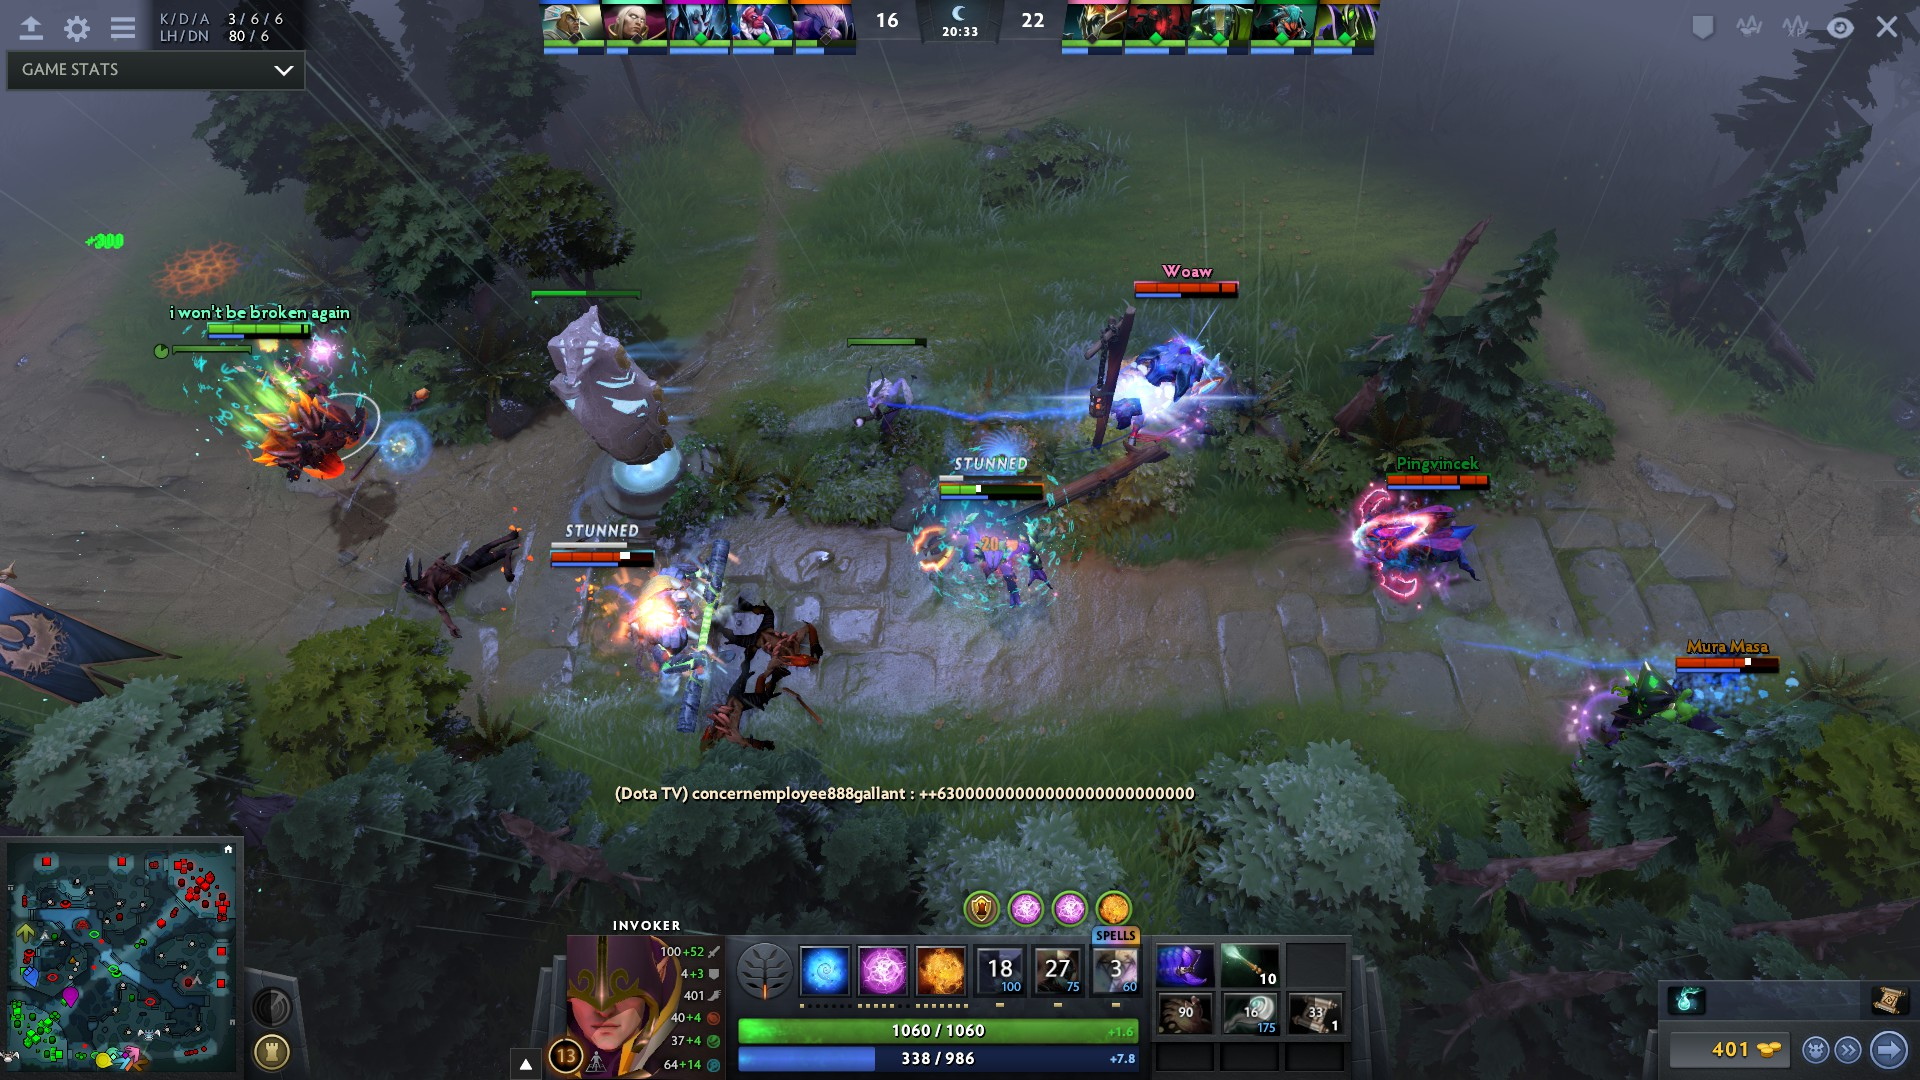
\includegraphics[width=\textwidth]{Cap4/dota.jpg}
    \caption{Dota 2: cena de batalha}
    \label{fig:dota}
\end{figure}

Um exemplo que pode ser citado é um jogo muito conhecido atualmente chamado Dota 2 \cite{dota}. Trata-se de um jogo de batalha \textit{online} onde dois times de 5 jogadores se enfrentam. Cada jogador controla seu personagem em seu próprio computador. A figura \ref{fig:dota} mostra uma cena de batalha do jogo e nos exemplifica as diversas variáveis que podereiam ser utilizadas para a geração dos valores instantâneos de entropia. São elas: valor da vida do personagem controlado, distância deste aos personagens aliados, distância aos personagens inimigos, quantidade de vida dos aliados e inimigos, tempo de jogo, quantidade de dano deferida nos últimos momentos, etc. Assim, é possivel imergir o jogador em uma música de acompanhamento que tente ilustrar sonoramente o que está acontecendo na partida que está sendo disputada assim como a interação entre os jogadores.
